% This is samplepaper.tex, a sample chapter demonstrating the
% LLNCS macro package for Springer Computer Science proceedings;
% Version 2.20 of 2017/10/04
%
\documentclass[runningheads]{llncs}
%
\usepackage{graphicx}
% Used for displaying a sample figure. If possible, figure files should
% be included in EPS format.
%
% If you use the hyperref package, please uncomment the following line
% to display URLs in blue roman font according to Springer's eBook style:
% \renewcommand\UrlFont{\color{blue}\rmfamily}
\usepackage[dvipsnames]{xcolor}
\usepackage{amsmath}
\usepackage{graphicx}
\usepackage{caption}
\usepackage{flafter}
\usepackage[colorlinks=true, allcolors=blue]{hyperref}
\usepackage{hyperref}
\usepackage{xcolor}
\usepackage{minted}
\begin{document}
	%
	\title{Mersul Trenurilor - Raport tehnic}
	%
	%\titlerunning{Abbreviated paper title}
	% If the paper title is too long for the running head, you can set
	% an abbreviated paper title here
	%
	\author{Șorodoc Tudor-Cosmin \\ (Grupa A4)}
	\date{06 Decembrie 2022}
	\institute{Universitatea "Alexandru Ioan Cuza"}
	%
	\maketitle              % typeset the header of the contribution
	%
	\begin{center}
		\keywords{sockets  \and threads \and database}  
	\end{center}
	\par\noindent\rule{\textwidth}{0.4pt}
	\section{Introducere}
	\subsection{Despre aplicație}
	Aplicația \textbf{Mersul trenurilor}, așa cum face referire și numele acesteia,
	oferă posibilitatea utilizatorilor de a afla informații despre traseul unor trenuri
	( orele la care acestea ajung într-o anumită stație, dacă au întârziere, dacă nu cumva mersul unui tren a fost anulat,...etc).
	\subsection{Utilizare}
	Aplicația pune la dispoziția utilizatorilor un \textbf{meniu}, prin care aceștia pot afla diverse informații, și anume :
	\begin{itemize}
		\itemsep0em
		\item Orele la care ajung trenurile într-o stație $" X "$ (specificată de utilizator) în data de $"D"$ (de asemenea, specificată de utilizator) și în traseul acestor trenuri, trec și prin stația $"Y"$;
		\item Trenurile care pleacă în urmatoarea oră, (și întârzierea cu care pleacă, dacă este cazul) dintr-o stație $"X"$;
		\item Trenurile care sosesc în urmatoarea oră, (și dacă ajung mai devreme sau cu întârziere ) într-o stație $"X"$;
		\item De asemenea, în meniul aplicației apare și opțiunea de a alege comanda de \textit{login};
		Un utilizator se va putea loga, doar dacă acesta este Administrator(i.e. utilizatorii normali nu au acces la un username si la o parola prin care s-ar putea conecta).\\
		Un Administrator va avea în meniul aplicației, bineînțeles după ce s-a logat, pe lângă opțiunile pe care le are un utilizator normal, și comenzi prin care :
		\begin{itemize}
			\itemsep0em
			\item poate adăuga un nou tren, cu traseul acestuia;
			\item poate introduce întârzierea pe care o are un tren $"T"$, la sosirea/plecarea în/din stația $"X"$; cu alte cuvinte, Administratorii sunt singurii care pot modifica baza de date;
			\item poate crea un cont nou de administrator, cont care poate fi utilizat de alt utilizator;
			\item poate schimba username-ul/parola;
			\item poate da logout;
		\end{itemize}
	\end{itemize}
	\section{Tehnoligii utilizate}
	\subsection{TCP/IP}
	La baza sistemului de comunicare al aplicației stau protocoalele TCP/IP (Transmition Control Protocol/ Internet Protocol).
	TCP este un protocol orientat-conexiune, adică pentru transmiterea mesajelor între 2 host-uri este nevoie de realizarea unei conexiuni.
	Conexiunile TCP sunt full duplex și se realizează prin așa numitul \textbf{"three way handshaking"},
	astfel asigurând o confirmare de primire a datelor.
	Protocolul TCP garantează livrarea corectă a datelor la destinatar, fără pierderi sau duplicări.
	Aplicația folosește acest protocol întrucât păstrarea integrității  și a ordinii informațiilor trimise de la \textit{Server} către \textit{Client} este de o importanță majoră.
	Daca aplicația nu ar avea la bază o comunicare sigură, atunci ar exista riscul ca datele trimise de la Server la Client să fie alterate, astfel Clientul primind o dată/oră greșită cu privire la mersul unui tren.
	De asemenea, rapiditatea nu este esențială, cu alte cuvinte, Clientul ar prefera ca să primească un raspuns corect, într-un timp mai mare, decât unul rapid, dar posibil gresit.
	
	
	\subsection{MySQL}
	Aplicația presupune afișarea informațiilor cu privire la mersul trenurilor, deci trebuie să ținem evidența fiecărui tren, în ce stație ajunge, la ce oră, dacă are întârziere și la ce oră pleacă din stația respectivă.
	De asemenea, trebuie să stocăm parolele și username-urile administratorilor.
	Din aceste motive, este esențială utilizarea unei baze de date.
	MySQL este un sistem de gestiune a bazelor de date relaționale și se poate folosi impreună cu limbajul C/C++.
	\\ \\ \\ \\ \\ \\ \\ \\ \\ \\ \\ \\
	\section{Arhitectura aplicației}
	\begin{center}
		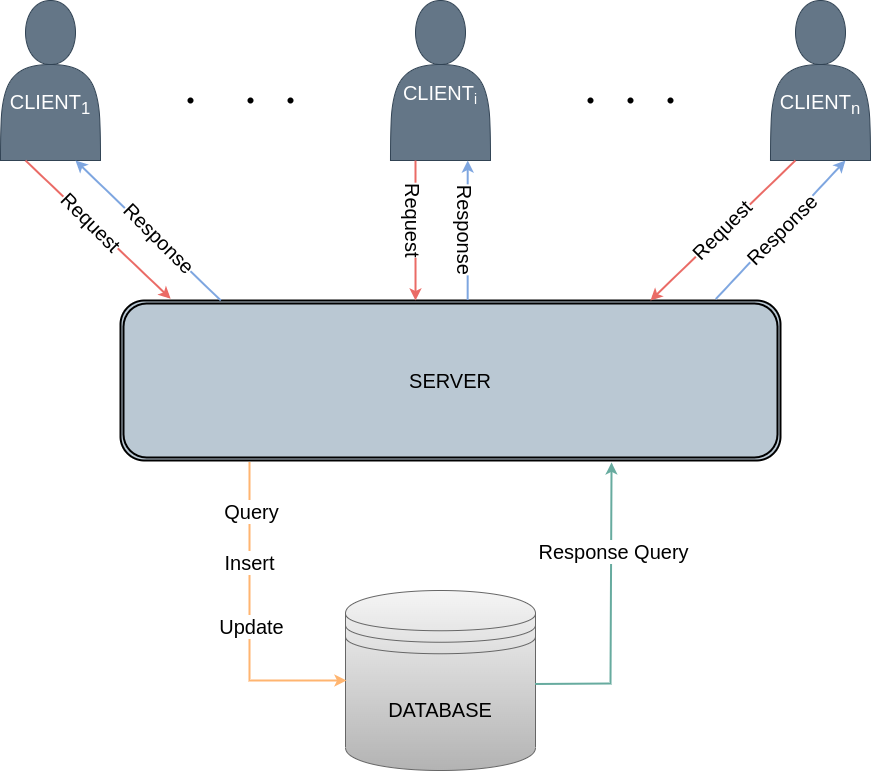
\includegraphics[scale=0.4]{diagram.png}
		\captionof{figure}{Diagrama generală a aplicației}
	\end{center}
	După cum se observă și în imaginea de mai sus, aplicația are la bază modelul $Client-Server$.
	În continuare, sunt prezentate diagrame mai detaliate, atât pentru $Client$, cât și pentru $Server$.
	\begin{center}
		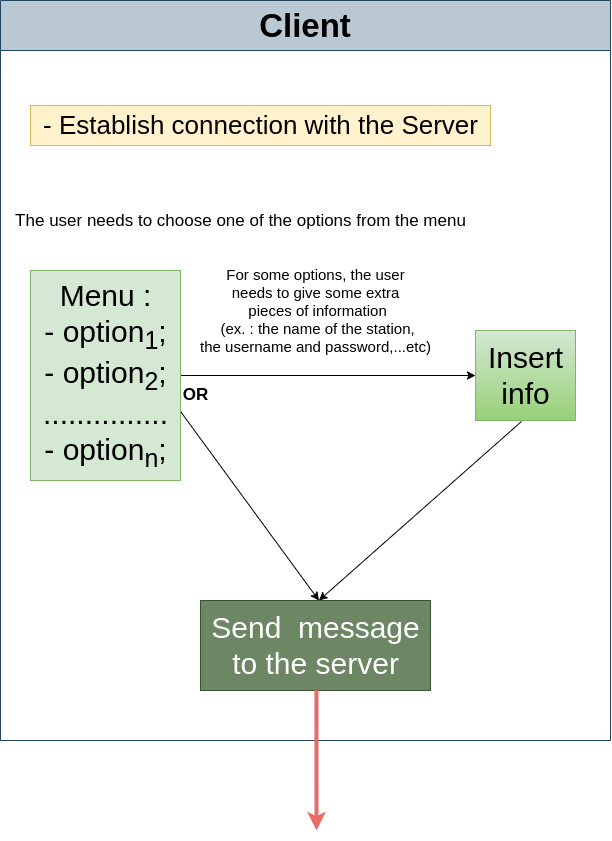
\includegraphics[scale=0.45]{diagram_client.png}
		\captionof{figure}{Diagrama - \textit{Client}}
	\end{center}
	Inițial $Clientul$ încearcă să stabilească \hyperlink{sec:detailsConnect}{o conexiune} cu $Serverul$, după care, daca s-a reușit conexiunea, îi afișează un meniu user-ului, din care poate alege diverse opțiuni.
	În fucție de opțiunea aleasă, user-ul trebuie să introducă date relevante pentru acea opțiune 
	(Ex: User-ul este de fapt, un Administrator și alege opțiunea de login. Alegând acestă opțiune user-ul trebuie să introducă un \textit{username} și o \textit{parolă}).
	Toate aceste date introduse de user sunt transmise prin intermediul unui \textbf{socket}("atașat" unui anumit $PORT$ și $adresa$ $IP$) către $Server$.
	
	\begin{center}
		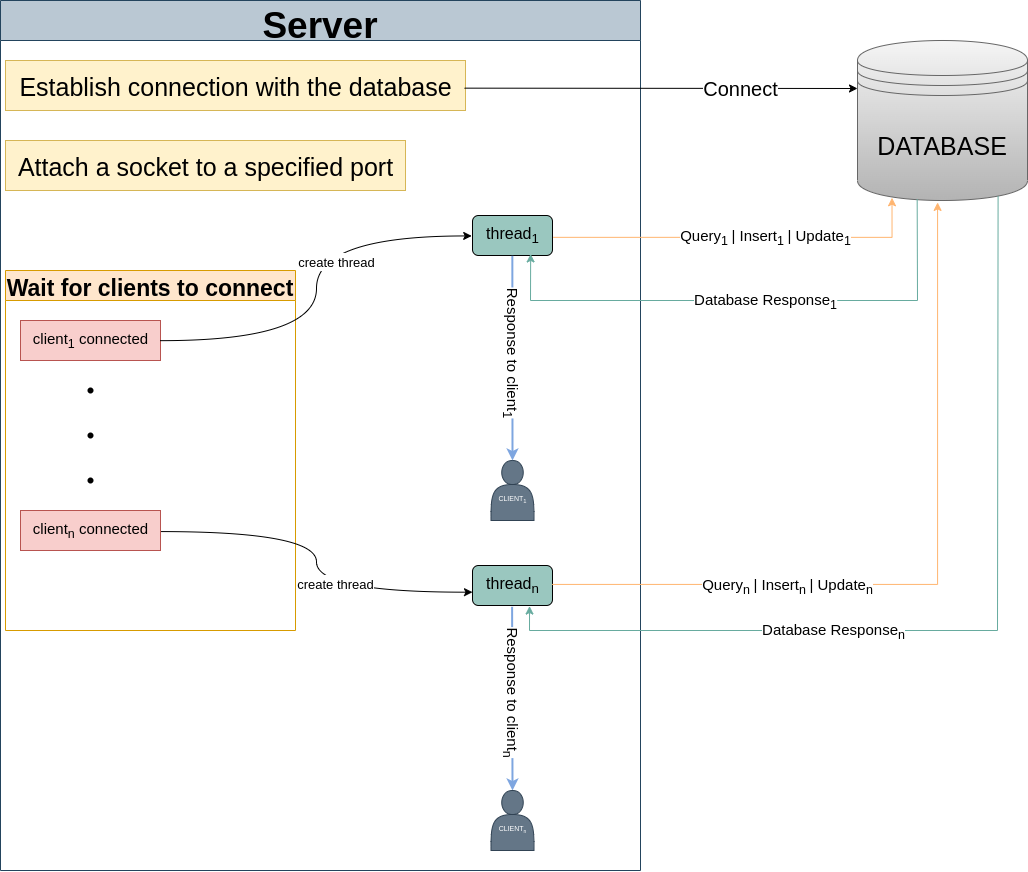
\includegraphics[scale=0.4]{diagram_server.png}
		\label{sec:server}
		\captionof{figure}{Diagrama - \textit{Server}}
	\end{center}
	Inițial $Serverul$ se conectează la o \hyperref[sec:ServerDataBase]{bază de date} care conține informațiile necesare pentru a răspunde cererilor Clienților.
	$Serverul$ atașează unui socket un port specific, socket care o să fie folosit de $Client$ pentru a comunica cu $Serverul$. 
	Într-o buclă infinită Serverul asteaptă conexiuni de la $Clienti$, iar în momentul în care se conectează un Client, se \hyperlink{sec:ServerCreateThread}{creează un \textbf{thread}} pentru acesta.
	În funcție de mesajul pe care îl primește $Serverul$ de la $Client$, se apelează funcții specifice care trimit un query bazei de date si primesc răspuns
	(Ex: Mesajul primit de Server corespunde comenzii de login, deci se va trimite catre baza de date un query de forma 
	"SELECT * from userTable WHERE usernames=usernameRecieved AND password=passwordRecieved").
	În funcție de rezultatul interogării, se trimite răspuns către $Client$.
	
	\section{Detalii de implementare}
	Așa cum am precizat și mai sus, comunicarea între Clienți și Server se face prin socket-uri.
	\begin{minted}{c++}
		/* create the socket */
		if ((sd = socket (AF_INET, SOCK_STREAM, 0)) == -1){
			perror ("Socket Error.\n");
			return errno;
		}
	\end{minted} 
	AF\_INET - specifică familia de protocoale cu care va comunica socket-ul, și anume IPv4;\\
	SOCK\_STREAM - tipul socket-ului va fi TCP (transmisie sigură);\\
	
	\subsection{Client}
	\hypertarget{sec:detailsConnect}{$Clientul$} se conectează la $Server$ prin primitiva \textit{connect()}:
	\begin{minted}{c++}
		/* connect to the Server */
		if (connect (sd, (struct sockaddr *) &server,sizeof (struct sockaddr)) == -1){
			perror ("[-]Connect() Error.\n");
			return errno;
		}
	\end{minted}
	Bineînțeles, pentru ca această conexiune să se poată stabili, $Serverul$ trebuie sa fie pornit.\\
	User-ul trebuie să aleagă o opțiune din meniul dat, iar în funcție de opțiunea aleasă se apelează funcții specifice, care fie îi cer user-ului să mai introducă date, fie trimit \textit{request} către $Server$.\\
	După acest \textit{request}, Clientul asteaptă sa primească un $response$ de la $Server$, care va fi afișat pentru a fi văzut de user :
	\begin{minted}{c++}
		if ((nr_read=read (sd, buffer,sizeof(buffer))) < 0){
			perror ("[-]Read() Error, couldn't read the response from the server.\n");
			return errno;
		}	
		
		buffer[nr_read]='\0';	
		
		printf ("[+]The response is: %s\n", buffer);
	\end{minted}
	
	\subsection{Server}
	Serverul se conecteaza la baza de date : 
	
	\begin{minted}{c++} 
		
		SQL BD;
		
		if(BD.connect_to_databse() == false){//connect the server to the databse
			printf("[-]The server couldn't connect to the databse!\n);
			printf("! Try to restart the server ! \n");
			return -1;
		}
		else{
			printf("[+] The server connected to the databse successfully \n");
		}
	\end{minted} 
	Unde \textbf{SQL} este o clasă definitiă astfel : 
	\begin{minted}[frame=lines,
		framesep=2mm,
		baselinestretch=1.2,
		bgcolor=black!4,
		fontsize=\footnotesize,
		linenos]{C++}
		class SQL {
			private :
			MYSQL *connection;
			const std::string server_IP, username, password, database_name;
			public :
			SQL();//the constructor
			
			const std::string getServer_IP();
			const std::string getUsername();
			const std::string getDatabaseName();
			const std::string getPassword();
			
			bool connect_to_databse();
			
			MYSQL * getConnection();
			//^-returns the connection with the database
			MYSQL_RES* execute_query (std::string cmd_query);
			//^-returns the result of the query as MYSQL_RES*
			std::string get_result_of_the_executed_query();
			//^-this functions will be called after the execute_query();
			//it returns the result of the query as a string
		};
	\end{minted}
	\\
	\\
	\\
	\\
	\\  
	\\
	\\
	\hypertarget{sec:ServerCreateThread}{$Serverul $} va trata clienții concurent, folosind thread-uri : 
	\begin{minted}[frame=lines,
		bgcolor=black!4
		]{C++}
		/* Accept a client (blocking state untill a client connects*/
		if ( (client = accept (sd, (struct sockaddr *) &from, (socklen_t*)&length)) < 0){
			perror ("[-]Accept() Error\n");
			continue;//the client will have to try to connect again
		}
		treat_client CLIENT(client, BD.getConnection());
		CLIENT.create_thread();
	\end{minted}
	Se poate observa faptul că instanța CLIENT, va avea in componența sa descriptorul către care trebuie să scrie $Serverul$ pentru a-i răspunde acestui client și conexiunea cu baza de date.
	Funcția $create\_thread$ din cadrul clasei \textbf{treat\_client}: 
	\begin{minted}[frame=lines,
		bgcolor=black!4]{C++}
		void treat_client::create_thread(){			
			pthread_t t;
			pthread_create(&t,NULL,worker_thread, this);		
		}
	\end{minted}
	Thread-ul creat va executa functia $worker\_thread$ și va avea ca parametru 
	întreaga instață (\textbf{this}). În cadrul aceste funcții se va citi $Request-ul$ primit de la $Client$ și în funcție de acesta, se vor apela unele funcții specifice. După ce se va obține $Respons-ul$, acesta va fi trimis la $Client$.
	\begin{minted}[frame=lines,
		bgcolor=black!4
		]{C++}
		if (write (ds_cl, result, sizeof(result)) <= 0){
			// where ds_cl = ((treat_client*)arg)->desciptor_client;
			perror ("[Thread]Write() Error. The response couldn't be send to the client\n");
			quit=1;//if the client leaves before getting an answer
		}
		else
		printf ("[Thread] The response was successfully sent.\n");
	\end{minted}
	
	\subsection{MySQL}
	Baza de date conține 3 tabele :
	\begin{enumerate}		
		\itemsep0em
		\item users; care are câmpurile :
		\begin{enumerate}
			\itemsep0em
			\item username(VARCHAR(20));
			\item password(VARCHAR(30)) ;
		\end{enumerate}
		\item trains; care are campurile : 
		\begin{enumerate}
			\itemsep0em
			\item id\_train(VARCHAR(5) și este cheie primară);
			\item additional\_infomartion (VARCHAR(50)) unde se poate specifica daca un tren este Anulat;
		\end{enumerate}
		\item arrivals\_departures; care are câmpurile :
		\begin{enumerate}
			\itemsep0em
			\item station\_name(VARCAHR(20));
			\item id\_train(VARCHAR(5));
			\item arrival(DATETIME);
			\item departure(DATETIME);
			\item delay(INT), dacă este negativ asta înseamnă ca trenul va ajunge cu $delay$ minute mai devreme in stație, dacă este pozitiv, asta înseamnă ca va ajune cu $delay$ minute mai târziu în stație și de asemenea, va pleca cu $delay$ minute mai târziu din stație, iar daca este NULL, atunci trenul ajunge și pleacă la ora deja stabilită;
		\end{enumerate}
	\end{enumerate}
	
	\section{Concluzii}
	Aplicația descrisă în paginile de mai sus ar putea fi îmbunătățită prin : 
	\begin{itemize}
		\item implementarea unei interfețe grafice;
		\item ștergerea automată a trenurilor din baza de date după un anumit interval de zile (nefiind necesară stocarea informațiilor a unor trenuri care deja au parcurs traseul lor);
		\item adăugarea login-ului și pentru userii normali, putând astfel să aleagă o nouă opțiune prin care ar selecta un tren pentru care să primească o notificare în cazul în care are întârziere, este anulat sau dacă sosește mai repede în stație;
		\item îmbunătățirea sistemului de login, și anume :
		\begin{itemize}
			\item la crearea unui cont, este necesară și introducerea adresei de email;
			\item în cazul in care un user își uită parola, aceasta poate fi recuperată/schimbată( serverul trimite un email cu un cod generat random, după care user-ul trebuie să introducă acel cod pentru a-și putea schimba parola);
		\end{itemize}
	\end{itemize}
	\section{Bibliografie}
	\begin{itemize}
		\item \url{https://zetcode.com/db/mysqlc/}
		\item \url{https://profs.info.uaic.ro/~ioana.bogdan/}
		\item \url{https://profs.info.uaic.ro/~computernetworks/files/7rc_ProgramareaInReteaIII_Ro.pdf}
		\item \url{https://dev.mysql.com/doc/c-api/8.0/en/c-api-function-descriptions.html}
		
	\end{itemize}
	
	
\end{document}
